\subsection{Optical Conductivity and Anisotropic Properties}

\begin{figure}
    \centering
    \begin{subfigure}{0.495\textwidth}
        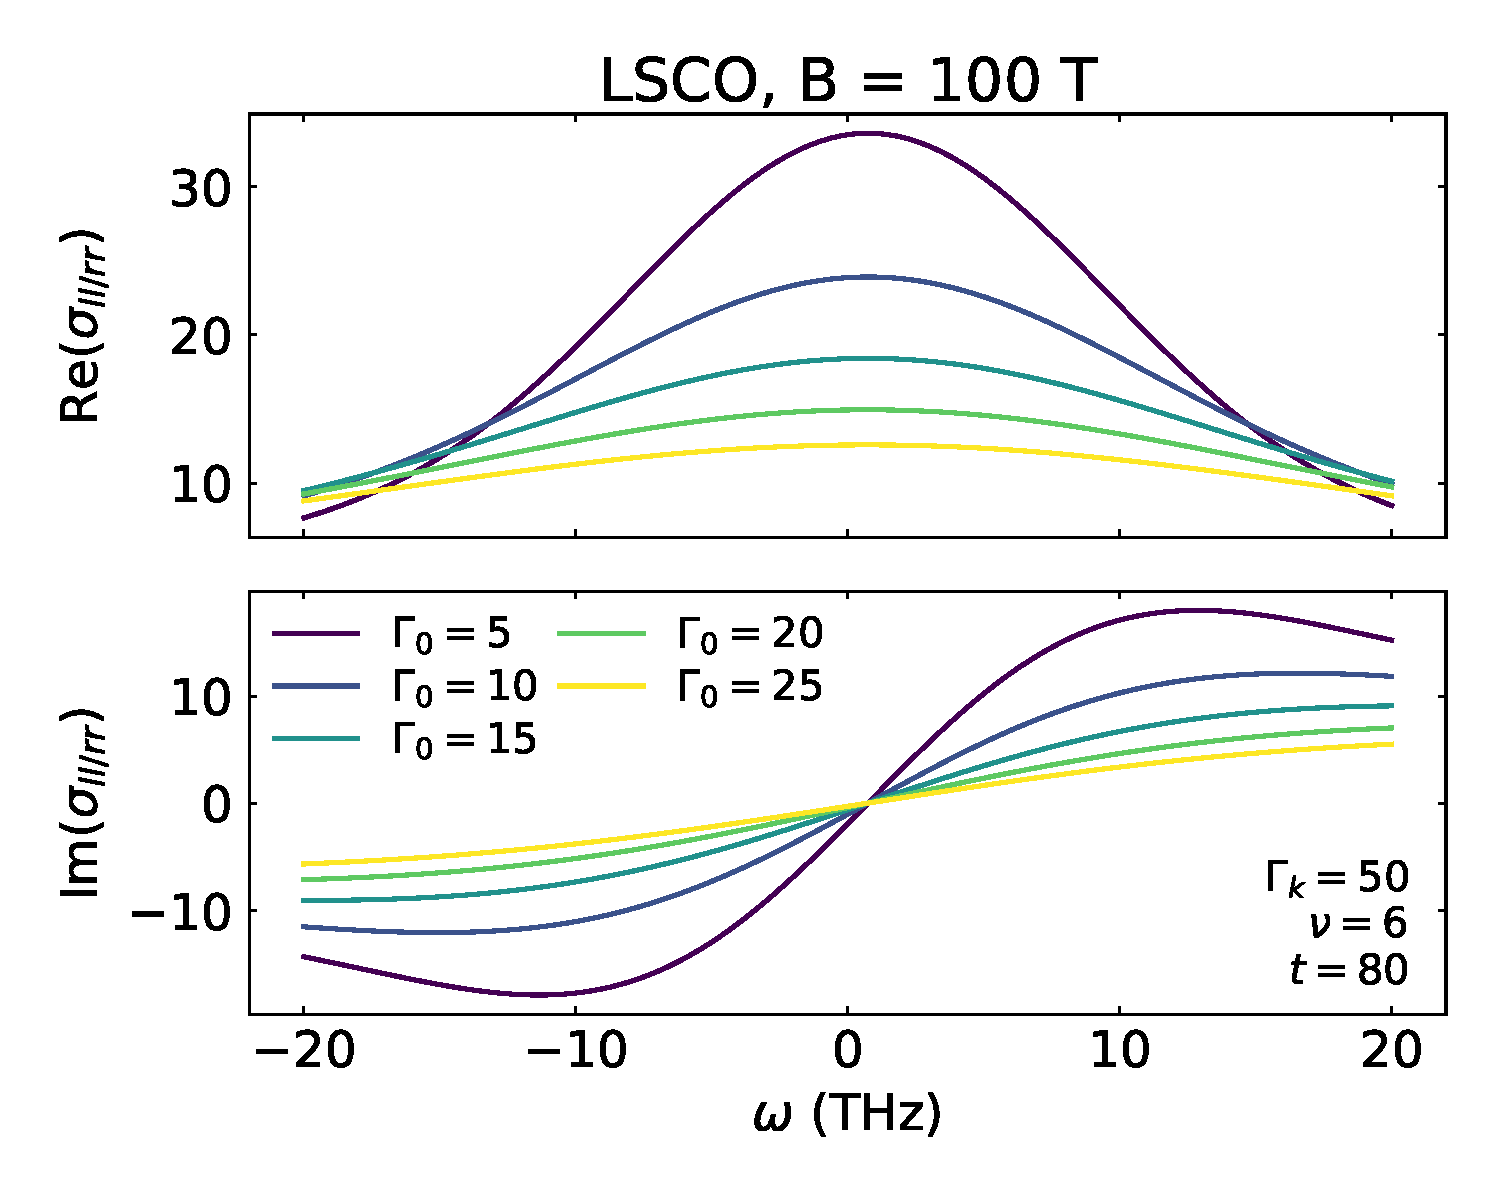
\includegraphics[width=\textwidth]{figures/vary_gamma_0}
        \caption{Varying the isotropic scattering rate}
        \label{fig:vary_gamma_0}
    \end{subfigure}
    \begin{subfigure}{0.495\textwidth}
        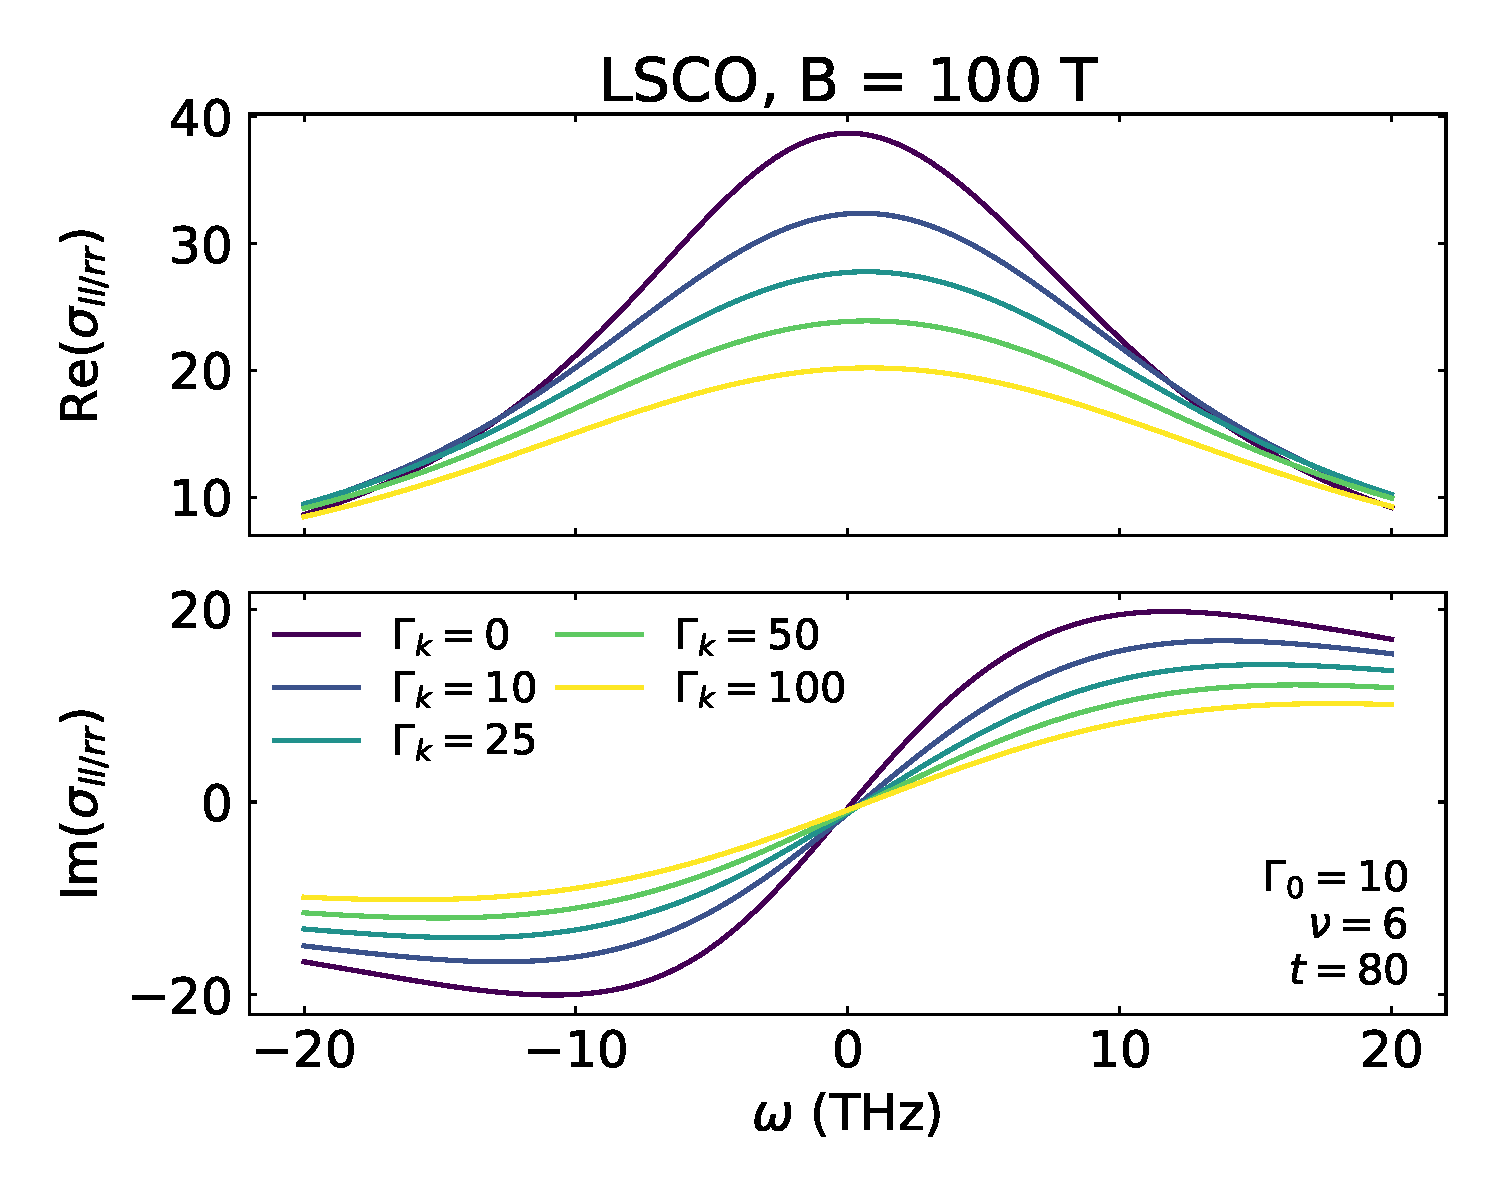
\includegraphics[width=\textwidth]{figures/vary_gamma_k}
        \caption{Varying the anisotropic scattering coefficient}
        \label{fig:vary_gamma_k}
    \end{subfigure}
    \begin{subfigure}{0.495\textwidth}
        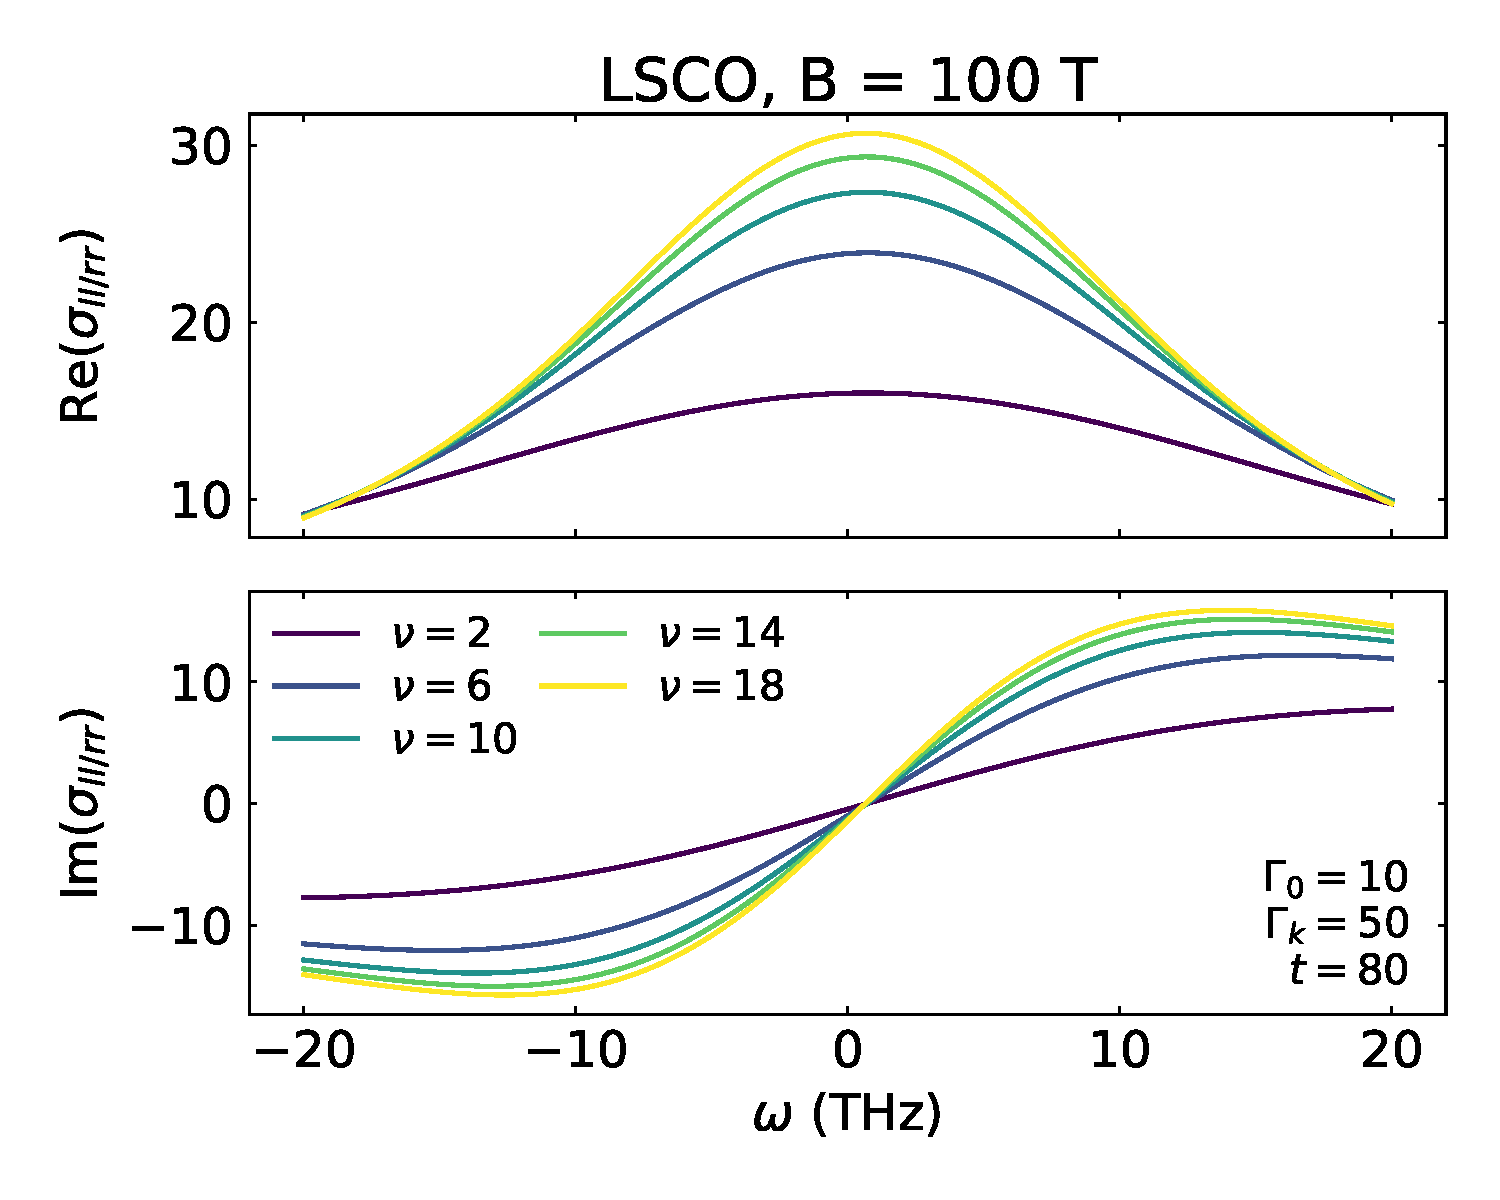
\includegraphics[width=\textwidth]{figures/vary_power}
        \caption{Varying the anisotropic scattering exponent}
        \label{fig:vary_power}
    \end{subfigure}
    \begin{subfigure}{0.495\textwidth}
        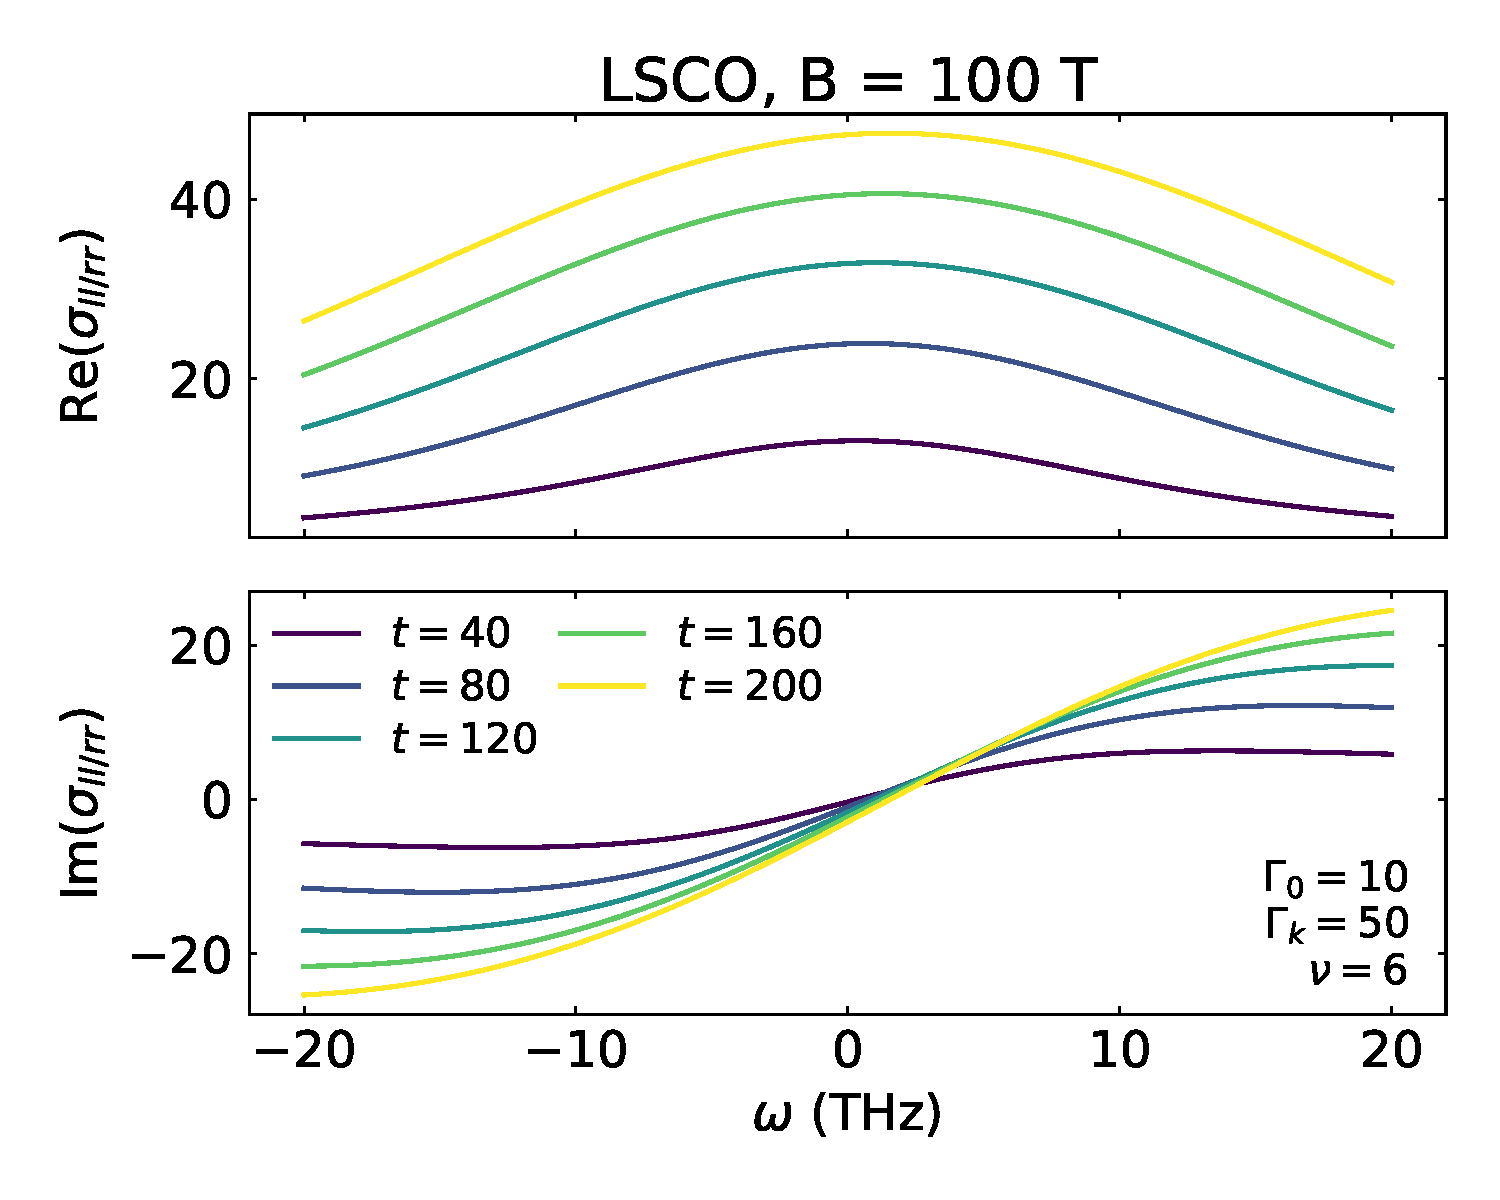
\includegraphics[width=\textwidth]{figures/vary_energy_scale}
        \caption{Varying the energy scale}
        \label{fig:vary_energy_scale}
    \end{subfigure}
    \caption{Effect of varying different model parameters}
    \label{fig:vary_parameters}
\end{figure}

\begin{figure}
    \centering
    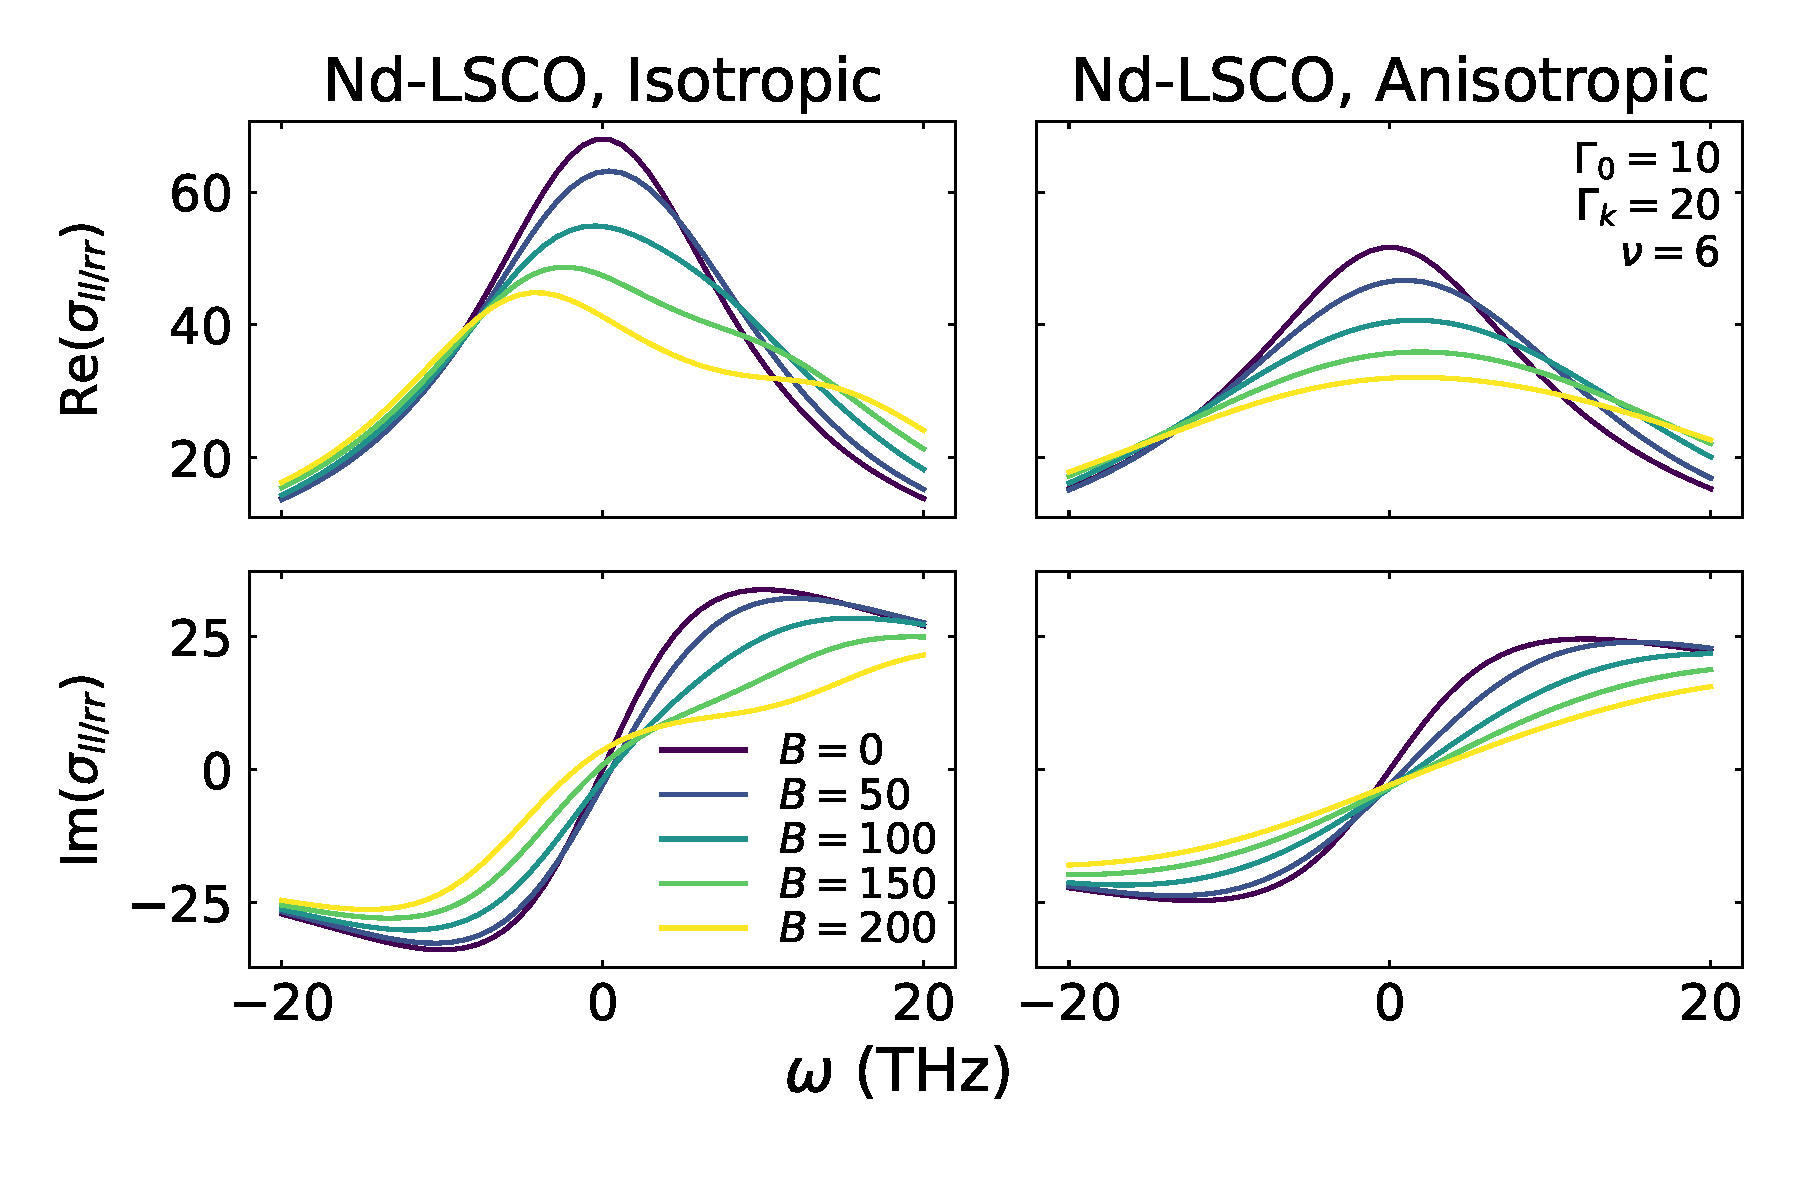
\includegraphics[width=0.7\textwidth]{figures/vary_field}
    \caption{Varying the magnetic field}
    \label{fig:vary_field}
\end{figure}

\begin{figure}
    \centering
    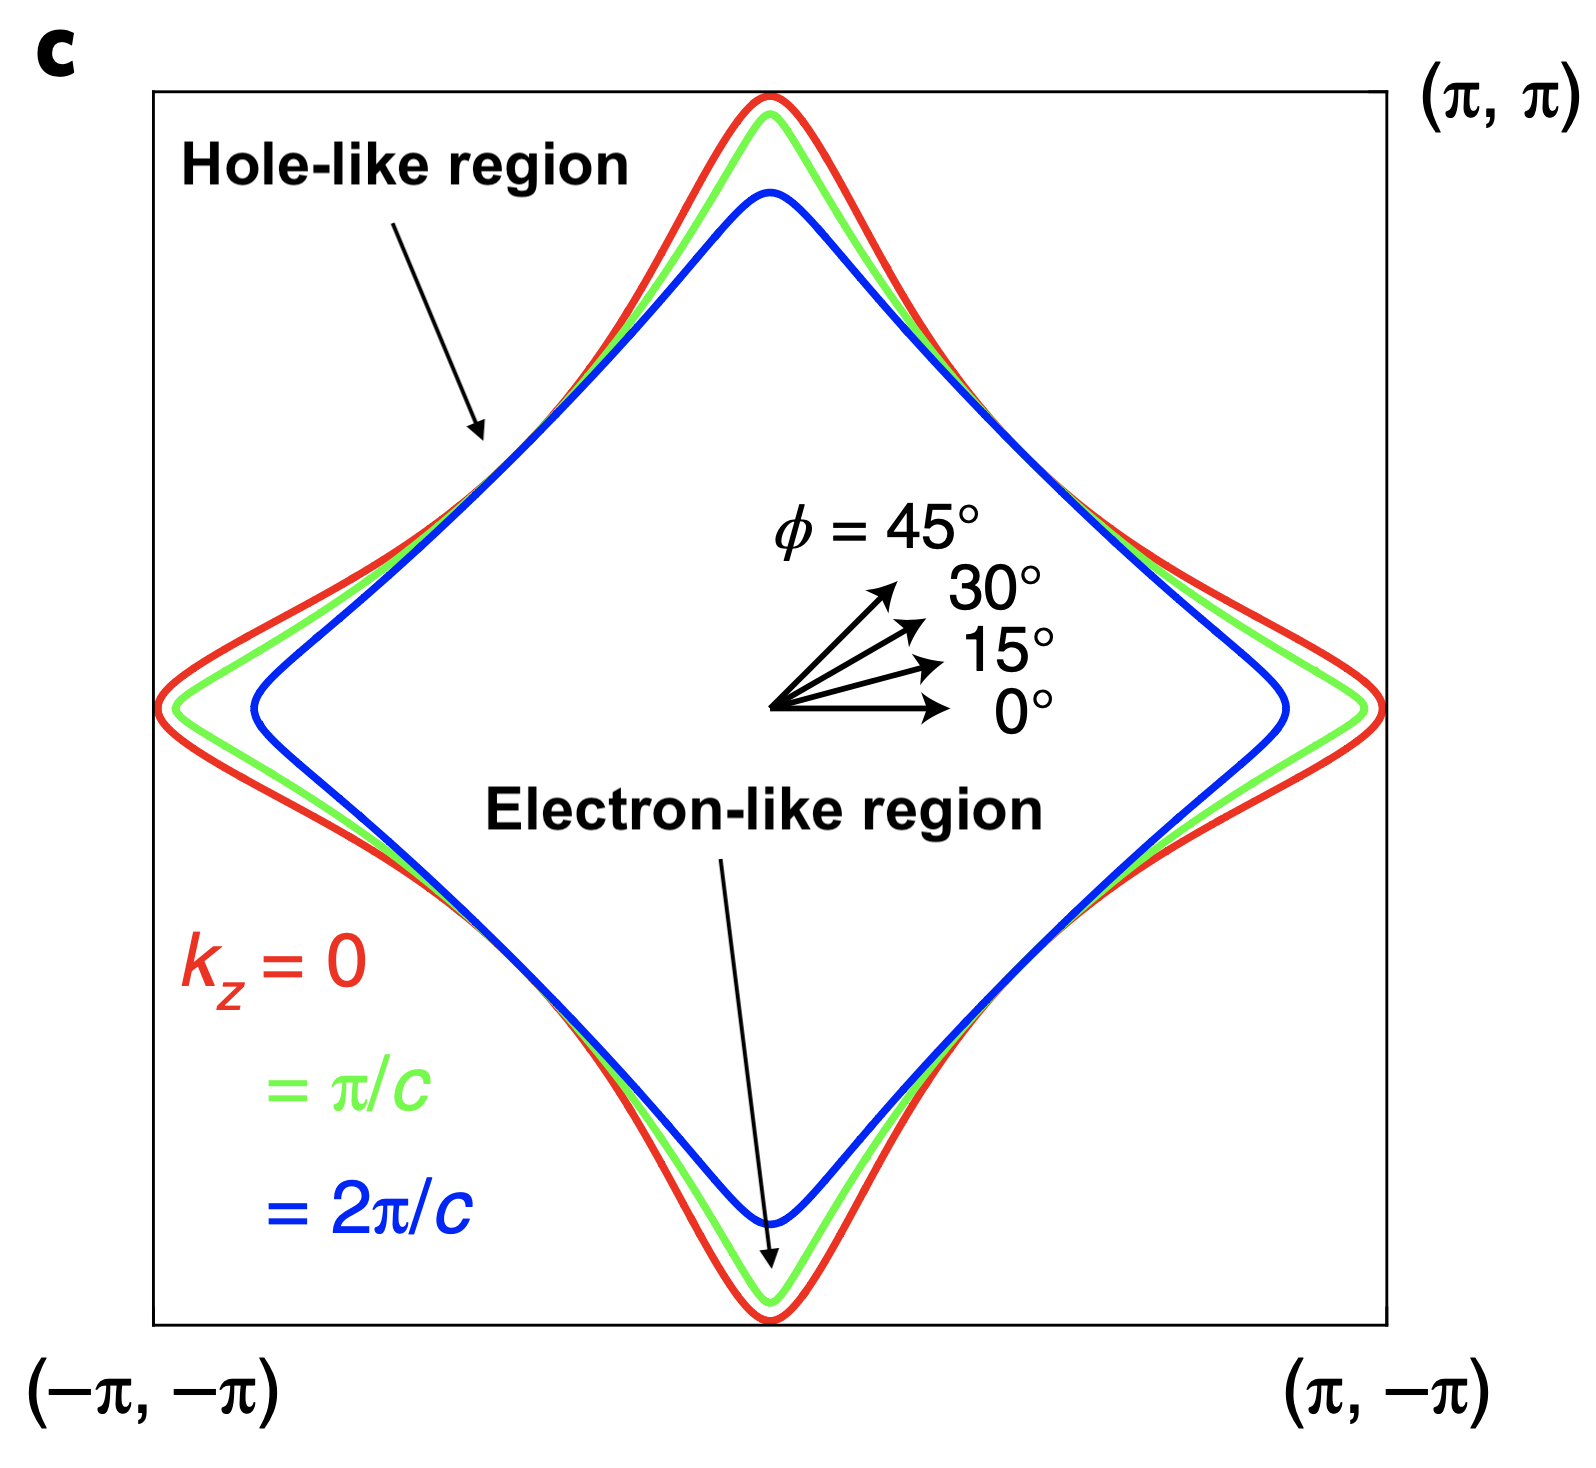
\includegraphics[width=0.7\textwidth]{figures/fermi_surface.png}
    \caption{From Fang et al.\cite{fang2022}, profile of the Fermi surface of NdLSCO at different $k_z$ slices}
    \label{fig:fermi_surface}
\end{figure}


Due to the complexity of the parameter space, 
we wanted to gain a qualitative understanding of the dependence of the conductivity curve on said parameters. 
To do that, we plotted the conductivity at fixed values for all but one parameter and observed the result
(Figure \ref{fig:vary_parameters}).

Looking at the effect of the different parameters in Figure, it seems each parameter roughly has
these effects:
\begin{itemize}
    \item Isotropic scattering rate ($\Gamma_0$): affects the overall magnitude of the conductivity
        and the width of the real conductivity peak (Figure \ref{fig:vary_gamma_0}).
    \item Anisotropic scattering coefficient ($\Gamma_k$): mostly affects the magnitude of the
        conductivity (Figure \ref{fig:vary_gamma_k}).
    \item Anisotropic scattering exponent ($\nu$): affects the shape of the real conductivity peak
        and greatly affects the magnitude of the conductivity (Figure \ref{fig:vary_power}).
    \item Energy scale: affects the magnitude of the conductivity and the position of the real
        conductivity peak, which means it affects the response of the peak to the magnetic field
        (Figure \ref{fig:vary_energy_scale}).
\end{itemize}

Figure \ref{fig:vary_field} shows the exagerated effect of the magnetic field on the conductivity.
As we increase the field, we see the conductivity peak splitting into one peak going into negative
$\omega$, and another into positive $\omega$. This is due to the different effect of the magnetic
field on the two different types of charge carriers in the material: negative (electron-like)
and positive (hole-like) particles.\footnote{The Fermi surface of LSCO has electron-like
and hole-like regions, defined by its curvature. This change in curvature flips a sign in the quadratic approximation of the dispersion relation used in the equations. See figure \ref{fig:fermi_surface}} A model with no anisotropic scattering would have two conductivity peaks,
one for each type of charge carrier. The anisotropic scattering would kill one of the peaks,
because it affects electron-like particles more severely. This is because of the different
electronic properties of the material for electron-like and hole-like particles.\footnote{
The electron-like region in LSCO's Fermi surface has far more anisotropy (i.e. curvature)
than the hole-like region. See figure \ref{fig:fermi_surface}.}

